\chapter{Functional Analysis}
\section{Hahn-Banach Theorem}
\subsection{The analytic form}
\begin{definition}
    A \textbf{poset} is a pair $(P,\leq)$, where $P$ is a set and $\leq$ is an ordered relation. A subset $C \subseteq P$ is said to be a \textbf{chain} if for all $x,y \in C$, either $x \leq y$ or $y \leq x$. 
\end{definition}
\begin{definition}
    A poset $(P,\leq)$ is said to be \textbf{inductively ordered} if any chain in $P$ has an upperbound in $P$.
\end{definition}
\begin{lemma}[Zorn]
    Any inductively ordered poset $(P,\leq)$ has a maximal element.
\end{lemma}
\begin{theorem}[Hahn-Banach]
    Let $p: E \to \bb{R}$ be a function satisfying 
    \begin{equation}
        \begin{cases}
            p(\lambda x) = \lambda p(x), \qquad\forall x \in E \text{ and } \forall \lambda >0,\\
            p(x + y) \leq p(x) + p(y),\qquad\forall x,y \in E.
        \end{cases}
    \end{equation}
    Let $G \subseteq E$ be a linear subspace and let $g: G \to \bb{R}$ be a linear functional such that 
    \[
        g(x) \leq p(x), \qquad x \in G.
    \]
    Then there exists a linear functional $f$ defined on $E$ that extends $g$ and such that 
    \[
        f(x) \leq p(x), \qquad x \in E.
    \]
\end{theorem}
\begin{proof}
    Consider the following set 
    \[
    P=\left\{h: D(h) \subset E \rightarrow \mathbb{R} \left\lvert\, \begin{array}{l}
D(h) \text { is a linear subspace of } E, \\
h \text { is linear, } G \subset D(h), \\
h \text { extends } g, \text { and } h(x) \leq p(x) \quad \forall x \in D(h)
\end{array}\right.\right\} .
    \]
    which the relation $\leq$ on $P$ satisfying
    \[
        h_1 \leq h_2 \lra D(h_1) \subseteq D(h_2) \text{ and $h_1$ extends $h_2$}.
    \]
    We claim that $P$ is inductively ordered, let $Q \subseteq P$ be a chain. Then one can write $Q = (h_i)_{i \in I}$ and set 
    \[
        D(h) = \bigcup_{i \in I}D(h_i) \text{ and $h$ extends every $h_i$}.
    \]
    Then it follows that $h \in P$ and $h$ is an upperbound of $Q$. Apply the Zorn lemma, one can obtain the maximal element $f \in P$. Now we claim that $D(f) = E$. Suppose for contradiction that $D(f) \neq E$, let $x_0 \in E \backslash D(f)$. Let $D(h) = D(f) \cup \{tx_0\mid t \in \bb{R}\}$ and $h(x + tx_0) = f(x) + t\alpha$, where $\alpha$ is some constant is chosen later to ensure that $h \in P$, in other words, we need to prove that 
    \[
        f(x) + t\alpha \leq p(x + tx_0) \qquad \forall x \in D(f) \text{ and }\forall t \in \bb{R}
    \]
    Equivalently, it suffices to find $\alpha$ such that 
    \[
        \sup_{t >0, x \in D(f)}\left\{\frac{f(x) - p(x - tx_0)}{t}\right\}\leq  \alpha \leq \inf_{t >0, x \in D(f)}\left\{\frac{p(x + tx_0) - f(x)}{t}\right\}
    \]
    Such $\alpha$ exits because since $f$ is linear, we have
    \[
        2f(x) = f(2x) \leq p(2x) \leq p(x - tx_0) + p(x  + tx_0)
    \]
    Thus $h \in P$ and $f < h$, which leads to contradiction since $f$ is maximal.  
\end{proof}
\begin{definition}
    Let $E^*$ be a dual space of $E$, we define the \textbf{dual norm} on $E^*$ by 
    \[
        \norm{f}_{E^*} =\sup_{\norm{x} \leq 1}\norm{f(x)}
    \]
\end{definition}
\begin{lemma}
    Let $G \subseteq E$ be a linear subspace. If $g: G \to \bb{R}$ is a continuous linear functional, then there exists $f \in E^*$ that extends $g$ and such that 
    \[
        \norm{f}_{E^*}= \norm{g}_{G^*}
    \]
\end{lemma}
\begin{proof}
    Apply Hahn-Banach theorem for $p(x) = \norm{g}_{G^8}\norm{x}$, then there exists $f \in E^*$ extending $g$ and
    \[
        f(x) \leq p(x) \lra \frac{f(x)}{\norm{x}} \leq \norm{g}_{G^*}
    \]
    This implies that $\norm{f}_{E^*} \leq \norm{g}_{G^*}$. But we already have that $\norm{f}_{G^*} = \norm{g}_{G^*}$. Hence $\norm{f}_{E^*} = \norm{g}_{G^*}$.
\end{proof}
\begin{lemma}
    For every $x_0 \in E$, there exists $f_0 \in E^*$ such that 
    \[
        \norm{f_0} = \norm{x_0} \text{ and }f(x_0) = \norm{x_0}^2
    \]
\end{lemma}
\begin{proof}
    Use lemma 8.6 with $G = \{tx_0 \mid t \in \bb{R}\}$ and $g(tx_0) = t\norm{x_0}^2$ so that $\norm{g}_{G^*} = \norm{x_0}$.
\end{proof}
\begin{lemma}
    For every $x \in E$, we have 
    \[
        \norm{x} = \sup_{f \in E^*, \norm{f} \leq 1}|f(x)| =\max_{f \in E^*, \norm{f} \leq 1}|f(x)| 
    \]
\end{lemma}
\begin{proof}
    We may assume that $x \neq 0$, since $f \in E^*$ is linear and $\norm{f} \leq 1$, it follows that 
    \[
        \sup_{f \in E^*, \norm{f} \leq 1}|f(x)|\leq \norm{x}
    \]
    By the lemma 8.7, there exists $f_0 \in E^*$ such that $\norm{f_0} = \norm{x}$ and $f_0(x)= \norm{x}^2$. Set $f_1 = f_0/\norm{x}$ then it follows that $\norm{f_1} = 1$ and $f_1(x) = \norm{x}$. Hence the following equality hold.
\end{proof}
\subsection{The geometric form}
\begin{definition}
    Let $E$ be a normed vector space, an \textbf{affine hyperplane} is a subset $H \subseteq E$ of the form 
    \[
        H := [f = \alpha]= \{x \in E \mid f(x) = \alpha\} 
    \]
\end{definition}
\begin{lemma}
    The hyperplane $H = [f = \alpha]$ is closed if and only if $f$ is continuous.
\end{lemma}
\begin{proof}
    If $f$ is continuous, then $H$ is clearly closed since $f^{-1}(\alpha)$ is closed. Now we suppose that $H$ is closed. Indeed, it suffices to prove that $f$ is bounded on $H^c$. Let $x_0 \in H^c$ so that $f(x_0) < \alpha$. Fix $r > 0$ such that $B(x_0,r) \subseteq H$. We claim that 
    \[
        f(x) < \alpha, \forall x \in B(x_0,r)
    \]
    Suppose $f(x_1) > \alpha$ for some $x_1 \in B(x_0,r)$. The segment
    \[
        L = \{x_t = (1 - t)x_0 + tx_1 \mid t \in [0,1]\}
    \]
    is contained  in $B(x_0,r)$, we need to find $t \in [0,1]$ such that 
    \[
        f(x_t) = \alpha \lra \alpha = (1 - t)f(x_0) + tf(x_1) \lra t = \frac{f(x_1) - \alpha}{f(x_1) - f(x_0)}
    \]
    Such $t$ is legal since $f(x_1) > \alpha$ and $f(x_0) < \alpha$, leads to contradiction. It follows that 
    \[
        f(x_0 + rz) < \alpha, \forall z \in B(0,1)
    \]
    or 
    \[
        f(z) < \frac{\alpha - f(x_0)}{r},\forall z \in B(0,1)
    \]
    Thus we obtain 
    \[
        \norm{f} = \sup_{x \in E, \norm{x} \leq 1}f(x) \leq \frac{\alpha - f(x_0)}{r} < \infty
    \]
    which implies that $f$ is continuous at $0$. Hence $f$ is continuous.
    \end{proof}
    \begin{definition}
        Let $A,B \subseteq E$. We say that the hyperplane $H = [f = \alpha]$ separates $A$ and $B$ if 
        \[
            f(x) \leq \alpha\quad \forall x \in A \quad \text{and}\quad f(x) \geq \alpha\quad\forall x \in B.
        \]
    \end{definition}
    \begin{definition}[Convex set]
        A subset $A \subseteq E$ is said to be \textbf{convex} if the segment
        \[
            \{tx + (1 - t)y \in A \mid x,y \in A, t \in [0,1]\} \subseteq A.
        \]
    \end{definition}
    \begin{center}
        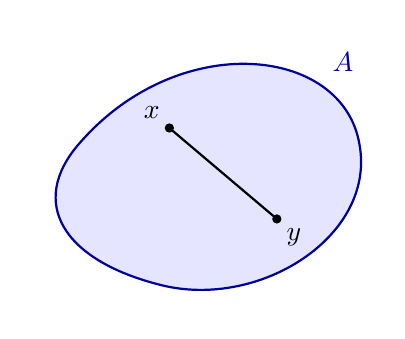
\begin{tikzpicture}[scale=1.05]
  % Convex set (blob)
  \fill[blue!10] (0,0)
    .. controls (1.2,1.4) and (3.2,1.2) .. (3.4,0)
    .. controls (3.6,-1.1) and (2.2,-2.0) .. (1.0,-1.7)
    .. controls (-0.2,-1.4) and (-0.6,-0.7) .. (0,0) -- cycle;
  \draw[blue!60!black, thick] (0,0)
    .. controls (1.2,1.4) and (3.2,1.2) .. (3.4,0)
    .. controls (3.6,-1.1) and (2.2,-2.0) .. (1.0,-1.7)
    .. controls (-0.2,-1.4) and (-0.6,-0.7) .. (0,0) -- cycle;

  % Points in the set
  \coordinate (x) at (1.1,0.2);
  \coordinate (y) at (2.4,-0.9);

  \fill (x) circle (1.6pt) node[above left] {$x$};
  \fill (y) circle (1.6pt) node[below right] {$y$};

  % Segment contained in the set
  \draw[thick] (x) -- (y);


  % Label
  \node[blue!60!black] at (3.2,1.0) {$A$};
\end{tikzpicture}
    \end{center}
\begin{theorem}[Geometric form of Hahn-Banach]
    Let $A,B\subseteq E$ be two nonempty disjoint convex subsets. Assume one of them is open. Then there exists a closed hyperplane that seperates $A$ and $B$.
\end{theorem}


\section{Picard-Lindelöf Theorem}
\begin{lemma}
    Let $K$ be a compact metric space and $(E,\norm{\cdot})$ be a Bannach space. Then the space $C(K,E)$ equipped with a suprenum norm $\norm{f}_{\infty} = \sup_{x \in K}\norm{f(x)}$ is Banach space.
\end{lemma}
\begin{proof}
    Let $\ep > 0$ be abitrary and $(f_n) \subseteq C(K,E)$ be a Cauchy sequence, then there exists $N \in \bb{N}$ such that $\norm{f_n - f_m}_{\infty}$ whenever $n,m > N$. Fix $x \in K$, then we have 
    \[
        \norm{f_n(x) - f_m(x)}_E \leq \norm{f_n - f_m}_{\infty} < \ep
    \]
    Then $(f_n)$ is Cauchy in $E$. Since $E$ is complete, there exists $f \in E$ such that $f_n \to f$. We claim that $f_n \to f$ uniformly. Fix $n > N$ and $x \in K$, then we have 
    \[
        \norm{f_n(x) - f(x)}_{E} = \lim_{m \to +\infty}\norm{f_n(x) - f_m(x)}\leq \lim_{m \to +\infty}\norm{f_n - f_m}_{\infty} \leq \ep
    \]
    Then $f_n \to f$ in $E$. In addition, taking $m \to \infty$ we obtain $\norm{f_n - f} \leq \ep$ for all $n \geq N$. Thus $f_n \to f$ in the sup norm. To prove $f \in C(K,E)$, fix $x_0 \in K$, we choose $N \in \bb{N}$ large enough such that 
    \[
        \norm{f -f_n}_{\infty} < \frac{\ep}{3} \text{ for all }n > N.
    \]
    Since $f_n$ is pointwise continuous, then there exists $\delta > 0$ such that $\norm{f_n(x) - f_n(x_0)}< \frac{\ep}{3}$ whenever $d(x,x_0) > \delta$. Then we obtain 
    \begin{align*}
        \norm{f(x) - f(x_0)} &\leq \norm{f(x) - f_n(x)} + \norm{f_n(x) - f_n(x_0)} + \norm{f_n(x_0) - f(x_0)}\\
        &\leq 2\norm{f - f_n}_\infty + \norm{f_n(x) - f_n(x_0)}\\
        &< \ep
    \end{align*}
    Since $x_0 \in K$ was abitrary, then $f \in C(K,E)$, which implies that $C(K,E)$ with the suprenum norm is a Banach space.
\end{proof}
\begin{theorem}[Banach Fixed Point theorem]
    Let $(X,d)$ be a complete metric space, $q \in [0,1)$ and $T: X \to X$ be a mapping on $X$ satisfying
    \[
         d(T(x),T(y)) \leq qd(x,y) \text{ for all }x,y.
    \]
    Then $T$ admits a unique fixed point $x^*$ in $X$.
\end{theorem}
\begin{proof}
    Let $x_0 \in X$ be abitrary and let $(x_n)$ be the sequence defined by $x_n = T(x_{n - 1})$ for all $n \geq 1$. Notice that for all $n \in \bb{N}$ we have we claim the estimate 
    \[
        d(x_m,x_n) \leq \frac{q^n}{1 - q}d(x_1,x_0)
    \]
    for all $m > n$ can be reached by using the inequality 
    \[
        d(x_{n + 1}, x_n)\leq q^nd(x_1,x_0), \text{ for all }n \in \bb{N}
    \]
    Let $\ep > 0$ be abitrary, then one can choose $N \in \bb{N}$ large enough such that $\frac{q^n}{1 - q}d(x_1,x_0) < \ep$. Thus $(x_n)$ is a Cauchy sequence, and since $X$ is complete, then $x_n$ coverges to some $x^* \in X$ and we obtain 
    \[  
        x^* = \nlim x_n = \nlim T(x_{n - 1}) = T(x^*)
    \]
    Thus $x^*$ is a fixed point in $X$. To prove the uniqueness, suppose $p_1 \neq p_2$ are two fixed point in $X$, then we have 
    \[
        d(p_1,p_2) = d(T(p_1),T(p_2)) \leq qd(p_1,p_2) < d(p_1,p_2),
    \]
    which is a contradiction, as desired.
\end{proof}
\begin{theorem}[Grönwall inequality]
    Let $u: [t_0,T] \to [0,\infty)$ be a continuous function, $C,L \geq 0$ and we have 
    \[
        u(t) \leq C + L\int_{t_0}^tu(s) ds \text{ for all } t \in [t_0,T]
    \]
    Then we have the estimate 
    \[
    u(t) \leq Ce^{L(t - t_0)}\text{ for all } t \in [t_0,T]
    \]
\end{theorem}
\begin{proof}
    Let $v(t) = C + L\int_{t_0}^tu(s) ds$ then we have $u(t) \leq v(t)$ and $v'(t) = Lu(t) \leq  Lv(t)$. Consider $w(t) = e^{-L(t - t_0)}v(t)$, differentiating $w$ yields 
    \[
         w'(t) = e^{-L(t - t_0)}(v'(t) - Lv(t)) \leq 0
    \]
    Thus $w(t) \leq w(t_0) = v(t_0) = C$, we obtain
    \[
        u(t) \leq v(t) \leq Ce^{L(t - t_0)}
    \]
    Hence we are done.
\end{proof}
\begin{theorem}[Picard-Lindelöf Theorem]
    Consider the Cauchy problem 
    \begin{equation}
        \begin{cases}
        x(t_0) = x_0,\\
        x'(t) =F(t,x(t))
    \end{cases}
    \end{equation}

    Let $U \subseteq \bb{R} \times \bb{R}^n$ be a closed set and $F: U \to \bb{R}^n$ be a continuous function in $t$, locally Lipchitz in $x$, i.e for every compact set $K \subseteq U$, there exists a local constant $L > 0$ such that
    \[
        \norm{F(t,x) - F(t,y)}\leq L\norm{(t,x) -(t,y)}
    \]
    for all $(t,x), (t,y) \in K$. Then there exists an interval $I$ containing $t_0$ and a unique solution $x \in C^1(I, \bb{R}^n)$.
\end{theorem}

\begin{proof}[Proof of the theorem]
    Let $a, r \in \bb{R}$ such that $r > 0$ and $W = [t_0 - a,t_0 +a] \times \clo{B(x_0,r)} \subseteq U$. Since $W$ is closed and bounded, it is compact. Then $f$ is bounded on $W$. 
    
    Let $M = \sup_{(t,x) \in M}\norm{f(t)}$, $h = \min\{\frac{b}{M}, \frac{1}{2L},a\}$ and $I = [t_0 -h, t_0 + h]$. We define the metric space $(X, \norm{\cdot}_{\infty})$
    \[
        X = \{x \in C(I,W) \mid \norm{x - x_0} \leq b\}.
    \] As $ C(I,W) \subseteq C^1(I, \bb{R}^n)$, $I$ is compact and $W$ is complete, then the above lemma follows that $C^1(I,W)$ is Banach. Since $X \subseteq C(I,W)$ is closed, then $X$ is also a Banach space. Integrating both sides of the second (6.1) yields
    \[
        x(t) = x_0 + \int_{t_0}^t F(x(s),s) ds
    \]
    Let $T: X \to C(I, \bb{R}^n)$ be the operator defined by $T[x] = x_0 + \int_{t_0}^t F(x(s),s) ds$. We claim that $T$ is invariant. Indeed, we have 
    \begin{align*}
        \norm{T[x] - x_0} = \norm{\int_{t_0}^t F(x(s),s) ds}\leq \int_{t_0}^t\norm{F(x(s),x)}ds \leq Mh \leq b
    \end{align*}
    Thus $T[x] \in X$. Futhermore, we aim to prove that $T$ is a contraction. Since $W$ is compact, then there exists $L > 0$ such that $f$ is Lipchitz with constant $L$ on $W$. Consider the following estimate 
    \begin{align*}
        \norm{(Tx)(t) - (Ty)(t)} &= \norm{\int_{t_0}^t F(x(s),s) - F(y(s),s)ds}\\
        &\leq \int_{t_0}^t\norm{F(x(s),s) - F(y(s),s)}ds\\
        &\leq L\int_{t_0}^t\norm{(x(s),s) - (y(s),s)}ds\\
        &\leq Lh\norm{x - y}\\
        &\leq \frac{1}{2}\norm{x - y}
    \end{align*}
    Taking the norm to suprenum yields $\norm{(Tx)(t) - (Ty)(t)} \leq \frac{1}{2}\norm{x - y}$. Thus $T$ is contraction. Apply the Banach Fixed Point theorem, then there exists unique $x^* \in X$ such that $T[x^*] = x^*$, or equivalently,
    \[
         x^*(t) = x_0 + \int_{t_0}^t F(x^*(s),s) ds
    \]
    Then $F(x^*(s),s)$ is continuous, the fudamental theorem implies that 
    \[
        \frac{d}{dt}x^*(t) = F(x^*(t),t).
    \]
    Hence $x^*$ is a solution $C^1(I,\bb{R}^n)$ of (6.1). To prove the uniqueness, suppose $x_1,x_2 \in C^1(I,\bb{R}^n)$ are solutions of (6.1), using the similar estimate we obtain
    \begin{align*}
        \norm{x_1(t) - x_2(t)} = \norm{(Tx_1)(t) - (Tx_2)(t)} \leq L \int_{t_0}^t\norm{x_1(t) - x_2(t)}ds
    \end{align*}
    If $t < t_0$, the RHS must vanish to zero, which implies that $\norm{x_1(t) - x_2(t)} = 0$ or $x_1(t) = x_2(t)$. If $t \geq t_0$, apply the Grönwall inequality for the function $u(t) = \norm{x_1(t) - x_2(t)}$, we obtain that $u(t) = 0$ for all $t \geq t_0$. Therefore $u_1(t) = u_2(t)$ for all $t \in I$, it follows that the existence of the solution $x^*$ in $C^1(I,\bb{R}^n)$ is unique.
    
\end{proof}
